\documentclass[10 pt,usenames,dvipsnames, oneside]{article}
\usepackage{../../../modelo-ensino-medio}



\begin{document}

\begin{center}
  \begin{minipage}[l]{3cm}

\includegraphics[width=2cm]{logo}    
\end{minipage}\hfill
\begin{minipage}[r]{.8\textwidth}
 {\Large \scshape Atividade: Círculo trigonométrico no GeoGebra}  
\end{minipage}
\end{center}
\vspace{.2cm}

% \ifdefined\prof
% %Habilidades da BNCC
% % \begin{objetivos}
% % \item 
% % \end{objetivos}

% %Caixa do Para o Professor
% \begin{goals}
% %Objetivos específicos
% \begin{enumerate}
% \item
% \end{enumerate}

% \tcblower

% %Orientações e sugestões
% \begin{itemize}
% \item 
% \end{itemize}
% \end{goals}

% \bigskip
% \begin{center}
% {\large \scshape Atividade}
% \end{center}
% \fi

Abra uma tela nova no GeoGebra e exiba os eixos coordenados. Construa os pontos $A(0,0)$ e $B(1,0)$ e construa o círculo de centro $A$ que passa por $B$.
\begin{enumerate}
\item Qual o raio dessa circunferência?
\item Quais os pontos de interseção entre a circunferência e os eixos coordenados? Quanto mede cada um dos arcos compreendidos entre esses pontos?
\item Os pontos que se localizam na circunferência cujas coordenadas são positivas são pontos que estão no $1$\super{o} quadrante. Faça uma figura indicando onde estão esses pontos. Da mesma forma, indique onde se localizam os que estão no $2$\super{o} quadrante (abscissa negativa e ordenada positiva), no $3$\super{o} quadrante (coordenadas negativas) e no $4$\super{o} quadrante (abscissa positiva e ordenada negativa).

\item Considere a reta real “enrolada”{} na circunferência conforme vimos no exercício anterior, com a mesma unidade dos eixos coordenados. Em que quadrante fica o número real $1$? E o número real $-1$? E o número real $\pi$? E o número real $\sqrt{2}$?
\item Marque um ponto $C$ sobre a circunferência de forma que o ângulo $B\hat{A}C$ meça $60^{\circ}$. Que número real está associado ao ponto C?
\end{enumerate}

\ifdefined\prof
\begin{solucao}

\begin{enumerate}
\item O raio da circunferência é 1.
\item  Os pontos são $(0,1)$, $(1,0)$, $(-1,0)$, $(0,-1)$. Os arcos podem ser $0\rad$, $\frac{\pi}{2}\rad$, $\pi\rad$ ou $\frac{3\pi}{2}\rad$, de acordo com quais pares de pontos estamos trabalhando.
\item Nesse item, espera-se que o aluno identifique os quadrantes.
\begin{figure}[H]
\centering

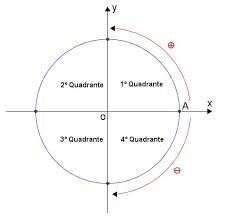
\includegraphics[width=.6\linewidth]{trigonometricas55}
\end{figure}

\item Podemos nos orientar, para responder a esse item, no valor decimal de $\pi$ como $3{,}14$. Então, dessa forma, temos: 
\begin{itemize}
\item $1$ está entre $0$ e $\frac{\pi}{2}$, logo, está no $1$\super{o} quadrante;
\item $-1$ está entre $\frac{-\pi}{2}$ e $0$, logo, está no $4$\super{o} quadrante ;
\item $\pi$ não está em nenhum quadrante pois está no eixo horizontal. 
\item $-\sqrt{2}$ vale aproximadamente $-1{,}4$, ou seja, está entre $-\frac{\pi}{2}$ e zero, portanto o quarto quadrante.
\end{itemize}
\item O ângulo de $60^{\circ}$ equivale a $\frac{1}{6}$ da volta inteira na circunferência, o que em radianos representa $\frac{1}{6}$ de $2\pi$, ou seja, $\frac{\pi}{3}$.
\end{enumerate}

\end{solucao}
\fi

\end{document}